\documentclass[12pt]{article}

\usepackage[utf8]{inputenc}
\usepackage[T1]{fontenc}      
\usepackage[english]{babel}
%\usepackage[left=2.00cm, right=2cm, top=2.00cm, bottom=2.00cm]{geometry}
\usepackage{amsthm}
\usepackage{fancyhdr}
\usepackage{amsmath}
\usepackage{amssymb}
\usepackage{mathrsfs}
\usepackage{stmaryrd} 
%\renewcommand{\qedsymbol}{}
\usepackage{graphicx}
\graphicspath{{illustrations/}}
\usepackage{caption}
\usepackage{dsfont}
\usepackage{xcolor}
\usepackage{textcomp}

\pagestyle{fancy}
\renewcommand{\headrulewidth}{1pt}
\lhead{}
\chead{\textsc{numerical simulation of sdes with distributional drift}}
\rhead{}

\newcommand{\pade}[2]{\frac{\partial #1}{\partial #2}}
\newcommand{\de}[2]{\frac{\mathrm{d} #1}{\mathrm{d} #2}}
\newcommand{\integ}[4]{\int_{#1}^{#2}{#3\ \mathrm{d} #4}}

\newtheorem{defi}{Definition}
\newtheorem{theo}{Theorem}
\newtheorem{lem}[theo]{Lemma}
\newtheorem{cor}[theo]{Corollary}
\newtheorem{Pro}{Proposition}
\newtheorem{ex}{Example}
\newtheorem{rem}{Remark}

\newcommand{\norme}[1]{\left\Vert #1\right\Vert}
\newcommand{\R}{\mathbb{R}}
\newcommand{\Z}{\mathbb{Z}}
\newcommand{\N}{\mathbb{N}}
\newcommand{\E}{\mathbb{E}}
\newcommand{\D}{D(\Omega)}
\newcommand{\Di}{D'(\Omega)}
\newcommand{\C}{\mathbb{C}}
\newcommand{\Cinf}{\mathcal{C}^\infty(\Omega,\R)}
\newcommand\gts[1]{\og#1\fg}
\newcommand{\n}{n\in\N^*}
\newcommand{\di}{\mathrm{d}}
\newcommand{\loc}{\mathcal{L}_{loc}^{1}(\Omega)}

\begin{document}
\title{\Large \textsc{\textbf{numerical simulation of sdes with distributional drift}}} \author{Maximilien \textsc{Germain} \date{May 2018}}
\maketitle

\section{Introduction}
    
    \paragraph{}
    We would like to simulate numerically sample paths of the solution of the stochastic differential equation
    \begin{equation} \label{sde}
    \di X_t = b(X_t)\ \di t + \di W_t
    \end{equation}
    where $b\in H^{-\beta}_q(\R),\ \beta\in\left(0,\frac{1}{2}\right)$, $q\in\left(\frac{1}{1-\beta},\frac{1}{\beta}\right)$, $t\in[0,T]$, and $W_t$ is a standard Brownian motion. Equation (\ref{sde}) is studied by F. Flandoli, E. Issoglio, and F. Russo in \cite{Fla-Iss-Rus-2017} in which they define a concept of virtual solution. The authors prove then existence and unicity in law of this solution. 
    
    \begin{ex}
        An example of such drift $b$ is given by the derivative of a sample path of a fractional Brownian motion $B^H_x$ with Hurst index $1/2<H<1$. These stochastic processes are gaussian processes verifying $$\E\left[B_t^HB_s^H\right]=\frac{1}{2}\left(t^{2H}+s^{2H}+|t-s|^{2H}\right).$$ We note $-\beta = H - 1$. Given $B^H_x(\omega)\in H^{1-\beta}_q(\R)$, we can take $b(x) = \pade{}{x}B^H_x(\omega)\in H^{-\beta}_q(\R)$. We will use this in our numerical simulations.
    \end{ex}    
    
    \paragraph{}
    As far as the drift $b$ is not a function but a distribution, it must be approximated if we want to evaluate it at points. In order to do so, we will use a series representation of $b$ and truncate it. That is why we will consider two steps in our algorithm: \begin{enumerate}
        \item approximate the drift $b$ by a function $b^N$ meant to converge to $b$ as $N\rightarrow\infty$.
        \item approximate the solution $X^N_t$ of the approximated SDE
        \begin{equation} \label{sde2}
        \di X^N_t = b^N\left(X^N_t\right)\ \di t + \di W_t
        \end{equation} 
        by $X^{N,n}_t$ defined with the Euler-Maruyama scheme
        \begin{equation*}
        X^{N,n}_t = X_0 + \int_0^t b^N\left(X^{N,n}_{\eta_n(t)}\right)\di t + W_{\eta_n(t)}
        \end{equation*}
        where $\eta_n(t)=t_k$ if $t\in[t_k,t_k+1]$, for $t_k=\frac{k}{n}$ with $ k\in\llbracket0,\lceil nT\rceil\rrbracket$.
        
    \end{enumerate}

\section{Numerical simulation of fractional Brownian motion}    
    \paragraph{}
    To simulate a sample path of a fractional brownian motion $B^H_x$ on a finite grid $(x_k)_{k\in\llbracket1,n\rrbracket}$, we simulate $n$ independent standard gaussian random variables $(X_k)_{k\in\llbracket1,n\rrbracket}$ and then correlate them with the definite positive correlation matrix 
    $$C_{k,s}=\E\left[B_{x_k}^HB_{x_s}^H\right]=\frac{1}{2}\left(x_k^{2H}+x_s^{2H}+|x_k-x_s|^{2H}\right).$$
    To do so, we use the Cholesky decomposition method and calculate the triangular matrix $M$ such that $C=MM^\top$. Therefore, defining
    $$X = \begin{pmatrix}
    X_1 \\ \vdots \\ X_n
    \end{pmatrix}\ \mathrm{and}\ B^H = MX,$$
    $B^H$ contains the values of a fractional brownian motion evaluated on the grid $(x_k)_{k\in\llbracket1,n\rrbracket}$.
    
\section{Approximation of the drift}
    \subsection{Series representation}
    \paragraph{}
    We use Haar wavelets to give a series representation of $b$. By doing so, we will be able to approximate it numerically by truncating the series.
    
    \begin{defi}[Haar wavelets]
        We define the Haar wavelets $h_{j,m}$ on $\R$ with $j\in\N\cup\{-1\}$ and $m\in\Z$ by:
        $$\begin{cases}
        h_M&:x\longmapsto\left(\mathds{1}_{\left[0,\frac{1}{2}\right[}-\mathds{1}_{\left[\frac{1}{2},1\right[}\right)(x)\\ h_{-1,m}&:x\longmapsto\sqrt{2}|h_M(x-m)|\\
        h_{j,m}&:x\longmapsto h_M(2^jx-m) 
        \end{cases}$$
    \end{defi}
    
    \begin{theo}[See \cite{Iss-Rus-2200}]
        Let $b\in H^s_q(\R)$ for $2\leq q \leq \infty$, and $s\in\left]-\frac{1}{2},\frac{1}{q}\right[$. Therefore,
        \begin{equation}
        b = \sum_{j=-1}^{+\infty}\sum_{m\in\Z}\mu_{j,m}h_{j,m}
        \end{equation}
        where $\mu_{j,m} = 2^j\int_{\R}b(x)h_{j,m}(x)\ \di x$ in the sense of dual pairing.
    \end{theo}

    \begin{defi}
        With the same notation $\mu_{j,m} $, let $b\in H^s_q(\R)$ for $2\leq q \leq \infty$, and $s\in\left]-\frac{1}{2},\frac{1}{q}\right[$. Given $N\in\N^*$ we define $b^N$ by:
        \begin{equation}
        b^N = \sum_{m=N}^{N-1}\mu_{-1,m}h_{-1,m}+\sum_{j=0}^{N}\sum_{m=-N2^j}^{N2^j-1}\mu_{j,m}h_{j,m}.
        \end{equation}
    \end{defi}

    \begin{rem}
        We can note that $\mathrm{Supp}\ b^N\subset [-N,N].$ Moreover, we have: $$\norme{b-b^N}_{H_q^s(\R)} \underset{N\rightarrow+\infty}{\longrightarrow} 0.$$
    \end{rem}

%    \subsection{Computation of the coefficients $\mu_{j,m}$ when $b$ is the derivative of a fractional brownian motion}
%        Faber basis

\newpage
\section{Convergence} 
    
    \subsection{Weak convergence of $X_T^{N,n}$ to $X_T^N$}
            \paragraph{}
            Recently, Leobacher and Szölgyenyi proved in \cite{Leo-Szo} the convergence of the Euler-Maruyama scheme for SDE with discontinuous but piecewise Lipschitz drift and with a degenerate diffusion coefficient. This framework applies to the scheme we use with piecewise constant drift $b^N$ and a constant diffusion coefficient.
    
       \begin{theo}[Theorem 3.1. in \cite{Leo-Szo}]\label{leo}
           $\exists C_N>0$ independent of $n$ such that it holds  $\forall \varepsilon >0,\ \exists n_0\in\N$, $\forall n\geq n_0$:
           \begin{equation}
            \E\left[\underset{0\leq t\leq T}{\sup}\left|X^{N,n}_t-X^N_t\right|^2\right]^{1/2}\leq C_N\delta^{1/4-\varepsilon}
            \end{equation}
            with $\delta=\frac{1}{n}$ the step size and $C_N$ depending on $\norme{b^N}_\infty$.
        \end{theo}
    
        \begin{theo}
            Let $f$ be $\mu$-Hölder with constant $C_f>0$ and $\mu\in(0,1]$. Then, exists $C_N'>0$ independent of $n$ such that it holds  $\forall \varepsilon >0,\ \exists n_0\in\N$, $\forall n\geq n_0$:
            \begin{equation}
            \left|\E\left[f\left(X_T^{N,n}\right)-f\left(X_T^N\right)\right]\right| \leq C_N'\delta^{\mu/4-\varepsilon}
            \end{equation}                       
            with $\delta=\frac{1}{n}$ the step size.
        \end{theo}
    
        \begin{proof}
            By Jensen's inequality and the $\mu$-Hölder property of $f$, we obtain:
            \begin{equation*}
            \left|\E\left[f\left(X_T^{N,n}\right)-f\left(X_T^N\right)\right]\right| \leq C_f  \E\left[\left|X_T^{N,n}-X_T^N\right|^\mu\right]
            \end{equation*}
            \begin{equation*}
             \leq  C_f  \E\left[\left|Y_T-Y_T^N\right|^2\right]^{\mu/2}
            \end{equation*}
            \begin{equation*}
            \leq C_f  C_N^\mu\delta^{\mu/4-\varepsilon}.
            \end{equation*}
        \end{proof}
    %\newpage
    
    \subsection{Weak convergence of $X^{N}_T$ to $X_T$}
        \paragraph{}
        The goal of this section is to estimate the weak error $\left|\E\left[f\left(X_T\right)-f\left(X_T^N\right)\right]\right|$ with suitable functions $f$. In order to do so, we must go back to the definition of the virtual solution of the SDE (\ref{sde}) given in \cite{Fla-Iss-Rus-2017}. Let $(\delta,p)\in K(\beta,q):=\{(\delta,p)\ |\ \beta<\delta<1-\beta,\ \frac{1}{\delta}<p<q\}$. The authors define the virtual solution of SDE (\ref{sde}) by $X_t$ such that:
        \begin{equation}\label{virtual}
        \begin{cases}
        Y_t = y + (\lambda+1)\int_0^t u(s,Y_s)\ \di s +\int_0^t (\nabla u(s,Y_s)+1)\ \di W_s \\X_t = \Psi(t,Y_t) = \varphi^{-1}(t,Y_t)
        \end{cases}
        \end{equation}
        where $u$ is the mild solution in $H_p^{1+\delta}$ of the following parabolic PDE:
        \begin{equation}\label{pde}
        \begin{cases}
        \partial_t u + \frac{1}{2}\Delta u + b\nabla u - (\lambda+1)u = -b\ &\mathrm{on}\ [0,T]\times\R\\
        u(T) = 0\ &\mathrm{on}\ \R
        \end{cases}
        \end{equation}
        and $\varphi(t,x) = x + u(t,x)$.
        
        \paragraph{}
        We also define another similar PDE by replacing $b$ by $b^N$. We call $u^N$ its mild solution in $H_p^{1+\delta}$:
        \begin{equation}\label{pde2}
        \begin{cases}
        \partial_t u^N + \frac{1}{2}\Delta u^N + b^N\nabla u^N - (\lambda+1)u^N = -b^N\ &\mathrm{on}\ [0,T]\times\R\\
        u^N(T) = 0\ &\mathrm{on}\ \R
        \end{cases}.
        \end{equation}
        Then we consider an approximated version of (\ref{virtual}): \begin{equation}\label{virtual approx}
        \begin{cases}
        Y_t^N = y + (\lambda+1)\int_0^t u^N\left(s,Y_s^N\right)\ \di s +\int_0^t \left(\nabla u^N\left(s,Y_s^N\right)+1\right)\ \di W_s\\
        X_t^N = \Psi^N(t,Y_t^N) = {(\varphi^N)}^{-1}(t,Y_t^N)
        \end{cases}.
        \end{equation}
        
        \begin{rem}
            Proposition 26 in \cite{Fla-Iss-Rus-2017} assures us that $X^N_t$ defined above in (\ref{virtual approx}) is in fact the classical solution of (\ref{sde2}), as far as $b^N\in L^p$. That is why for each fixed $N$ our Euler scheme converges to the virtual solution $X^N_t$.
        \end{rem}
    
    \paragraph{}              
    We also recall a useful lemma concerning the solutions of (\ref{pde}) and (\ref{pde2}).
    
    \begin{lem}[Lemma 20 in \cite{Fla-Iss-Rus-2017}]\label{lem}
        Let $(\delta,p)\in K(\beta,q)$ and let $u,\ u^N$ be the mild solution to (\ref{pde}) in $H_p^{1+\delta}$. Fix $\rho$ such that the integral operator is a contraction and let $\lambda>\rho$. Then $u(t),\ u^N(t)\in\mathcal{C}^{1,\alpha}$ with $\alpha=\delta-1/p$ for each fixed $t$ and 
        \begin{equation*}
        \begin{cases}
        \underset{(t,x)\in[0,T]\times\R}{\sup} |\nabla u(t,x)| \rightarrow 0,\ as\ \lambda \rightarrow \infty \\
        \underset{(t,x)\in[0,T]\times\R}{\sup} |\nabla u^N(t,x)| \rightarrow 0,\ as\ \lambda \rightarrow \infty
        \end{cases}
        \end{equation*}
        where the choice of $\lambda$ depends only on $\delta,\beta,\norme{b}_{H_p^{-\beta}}$, and $\norme{b}_{H_q^{-\beta}}$.
    \end{lem}
    
    \begin{lem}\label{morrey} Let $(\delta,p)\in K(\beta,q)$ and let $u,\ u^N$ be the mild solutions to (\ref{pde}),(\ref{pde2}) in $H_p^{1+\delta}$, $\alpha = \delta - 1/p$. Exists $c,K>0$ such that for both $N\in\N$ and $\rho>1$ big enough, $\forall t\in[0,T]$,
        \begin{equation}
        \begin{cases}
        \norme{u^N(t) - u(t)}_{L^\infty}\leq cKe^{\rho T}\norme{b^N-b}_{H^{-\beta}_{q}}\\        
        \norme{\nabla u^N(t) - \nabla u(t)}_{L^\infty}\leq c Ke^{\rho T}\norme{b^N-b}_{H^{-\beta}_{q}}.
        \end{cases} .
        \end{equation}
    \end{lem}    
    
    \begin{proof}
        Applying fractional Morrey inequality, $\exists c>0,\ \forall t\in[0,T]$:
        \begin{equation*}
        \begin{cases}
        \norme{u^N(t) - u(t)}_{L^\infty}\leq\norme{u^N(t) - u(t)}_{\mathcal{C}^{1,\alpha}}\leq c\norme{u^N(t)-u(t)}_{H^{1+\delta}_{p}}\\        
        \norme{\nabla u^N(t) - \nabla u(t)}_{L^\infty}\leq\norme{u^N(t) - u(t)}_{\mathcal{C}^{1,\alpha}}\leq c\norme{u^N(t)-u(t)}_{H^{1+\delta}_{p}}.
        \end{cases}        
        \end{equation*}        
        Now, we can conclude with
        \begin{equation*}
        \norme{u^N-u}_{\infty,H^{1+\delta}_{p}}\leq e^{\rho T} \norme{u^N-u}_{\infty,H^{1+\delta}_{p}}^{(\rho)}\leq Ke^{\rho T}\norme{b^N-b}_{H^{-\beta}_{q}}
        \end{equation*} from Lemma 23 in \cite{Fla-Iss-Rus-2017}, for both $N\in\N$ and $\rho>1$ big enough, and where $\norme{f(t)}_{\infty,X}^{(\rho)} := \underset{0\leq t\leq T}{\sup} e^{-\rho t} \norme{f(t)}_X$.
    \end{proof}
        
        \paragraph{}
        We will need the following local time inequality from Liqing Yan:        
        \begin{lem}[Lemma 4.2 in \cite{Yan}]\label{local}
            Let $X$ be a continuous semimartingale with $X_0 = 0$. For $\varepsilon>0$ we define a double sequence of stopping times by $\sigma_1 = 0$, $\tau_1=\inf\{t>0 | X_t=\varepsilon\}$, $\sigma_n = \inf\{t>\tau_{n-1}|X_t=0\}$, $\tau_n=\inf\{t>\sigma_n|X_t=\varepsilon\}$. For any real function $F(\cdot)\in\mathcal{C}^2$ with $F(0)=0,\ F'(0) = 0$ and $F(\cdot) > 0$ on $(0,\varepsilon_0)$ for some $\varepsilon_0 > 0$, then for any $0<\varepsilon<\varepsilon_0$ we have
            \begin{multline*}
                0\leq L^0_t(X) \leq 2\varepsilon - \frac{2}{F(\varepsilon)}\int_0^t \theta_s(X) \left(F\left(\varepsilon\right) - \varepsilon F'\left(X_s^+\right)\right)\ \di X_s\\
                +\frac{1}{F(\varepsilon)}\int_0^t \theta_s(X)\varepsilon F''(X_s^+)\ \di[X]_s
            \end{multline*}
            with $\theta_s(X) = \sum_{n=1}^\infty \mathds{1}_{\{\sigma_n< s\leq \tau_n,\ 0<X_s\leq \varepsilon\}}(X)$.
        \end{lem}        
        Applying lemma \ref{local} with $F(x) = x^2$, it follows:
        \begin{cor}\label{cor}
            Let X be a continuous semimartingale with $X_0 = 0$. With the same notations as in lemma \ref{local}, for any $\varepsilon>0$ we have
            \begin{multline}
                0\leq L^0_t(X) \leq 2\varepsilon - \frac{2}{\varepsilon}\int_0^t \theta_s(X) \left(\varepsilon - 2{X_s^+}\right)\ \di X_s
                +\frac{2}{\varepsilon}\int_0^t \theta_s(X) \ \di[X]_s
            \end{multline}
        \end{cor}

\begin{lem}\label{local time}
    Let $(\delta,p)\in K(\beta,q)$, $\alpha=\delta-1/p<1$, $u$, $u^N$ be the mild solutions to (\ref{pde}), (\ref{pde2}) in $H_p^{1+\delta}$, and $Y$, $Y^N$ solutions of the SDEs (\ref{virtual}), (\ref{virtual approx}).  Then, if $\alpha>1/2$, for $\lambda$ big enough we have $\forall\varepsilon\in(0,1]$,
    \begin{equation*}
    0\leq \E\left[L^0_T(Y-Y^N)\right]\leq  g(\varepsilon).
    \end{equation*}
    where \begin{multline*}
    g(\varepsilon) = 2(\lambda + 1)\ cT Ke^{\rho T}\norme{b^N-b}_{H^{-\beta}_{q}} + \left(4\norme{u}_{\mathcal{C}^{1,\alpha}}^2 T + 2+(\lambda + 1)T\right) \varepsilon^{2\alpha-1}\\
    + 4c^2T K^2e^{2\rho T}\norme{b^N-b}_{H^{-\beta}_{q}}^2\varepsilon^{-1}
    \end{multline*}
\end{lem}

\begin{proof}
    By Lemma \ref{lem}, we choose $\lambda$ big enough for $\nabla u$ and $\nabla u^N$ to be bounded by $\frac{1}{2}$. $\lambda$ can be chosen independently of $N$ as far as $\norme{b - b^N}_{H_q^s(\R)} \underset{N\rightarrow\infty}{\longrightarrow} 0$. Therefore $u^N(t,\cdot)$ and $u(t,\cdot)$ are $\frac{1}{2}$-lipschitz. We recall that in this case, by Lemma 22 in \cite{Fla-Iss-Rus-2017}, $\Psi(t,\cdot)$ is 2-lipschitz.
    Let $\varepsilon\in(0,1]$. Corollary \ref{cor} gives us:    
    \begin{multline*}
    0\leq L^0_T(Y-Y^N) \leq 2\varepsilon - \frac{2}{\varepsilon}\int_0^T \theta_s(Y-Y^N) \left(\varepsilon - 2{(Y_s-Y_s^N)^+}\right)\ \di (Y_s-Y_s^N)\\
    +\frac{2}{\varepsilon}\int_0^T \theta_s(Y-Y^N) \ \di[(Y-Y^N)]_s.
    \end{multline*}    
    \begin{rem}
        Note that $\theta_s(Y-Y^N) \left|\varepsilon - 2{(Y_s-Y_s^N)^+}\right|\leq \varepsilon\theta_s(Y-Y^N)$.
    \end{rem}
Let $t\in[0,T]$.
\begin{multline*}
Y_t-Y_t^N = (\lambda + 1 )\int_0^t\left\{u\left(s,Y_s\right)-u^N\left(s,Y_s^N\right)\right\}\ \di s\\ + \int_0^t\left\{\nabla u\left(s,Y_s\right)-\nabla u^N\left(t,Y_s^N\right)\right\}\ \di W_s.
\end{multline*}
%\begin{multline*}
%Y_t-Y_t^N = (\lambda + 1 )\int_0^t\left\{u\left(s,\Psi\left(s,Y_s\right)\right)-u^N\left(s,\Psi\left(s,Y_s^N\right)\right)\right\}\ \di s\\ + \int_0^t\left\{\nabla u\left(s,\Psi\left(s,Y_s\right)\right)-\nabla u^N\left(t,\Psi\left(s,Y_s^N\right)\right)\right\}\ \di W_s.
%\end{multline*}
%\begin{rem}  
%    For clarity purpose, we note $\tilde{u}\left(s,x\right) = u\left(s,\Psi\left(s,x\right)\right)$ and use the same notation for the gradient and the approximated mild solution. We can notice that $\tilde{u}$ is 1-lipschitz in space and $\widetilde{\nabla u}$ is $\alpha$-Hölder with constant $2\norme{u}_{\mathcal{C}^{1,\alpha}}$.
%\end{rem}
%$\widetilde{\nabla u}$ and $\widetilde{\nabla u}^N$ are bounded so the Itô integral is a martingale. We take the expectation:
${\nabla u}$ and ${\nabla u}^N$ are bounded so the Itô integral is a martingale. We take the expectation:
    \begin{multline*}
    \E\left[L^0_T(Y-Y^N)\right] \leq 2\varepsilon + 2(\lambda + 1)\ \E\left[\int_0^T\theta_s(Y-Y^N)\left\{u\left(s,Y_s\right)-u^N\left(s,Y_s^N\right)\right\} \di s \right]\\
    +\frac{2}{\varepsilon}\ \E\left[\int_0^T \theta_s(Y-Y^N)\left\{{\nabla u}\left(s,Y_s\right)-{\nabla u}^N\left(s,Y_s^N\right)\right\}^2\ \di s\right]
    \end{multline*}
    \begin{multline*}
    \leq 2\varepsilon + 2(\lambda + 1)\ \E\left[\int_0^T\theta_s(Y-Y^N)\left\{{u}\left(s,Y_s\right)-{u}\left(s,Y_s^N\right)\right\}\ \di s \right]\\+2(\lambda + 1)\ \E\left[\int_0^T\theta_s(Y-Y^N)\left\{{u}\left(s,Y_s^N\right)-{u}^N\left(s,Y_s^N\right)\right\}\ \di s \right]\\
    +\frac{4}{\varepsilon}\ \E\left[\int_0^T \theta_s(Y-Y^N)\left\{{\nabla u}\left(s,Y_s\right)-{\nabla u}\left(s,Y_s^N\right)\right\}^2\ \di s\right]\\
    +\frac{4}{\varepsilon}\ \E\left[\int_0^T \theta_s(Y-Y^N)\left\{{\nabla u}\left(s,Y_s^N\right)-{\nabla u}^N\left(s,Y_s^N\right)\right\}^2\ \di s\right]
    \end{multline*}
    \begin{multline*}
    \leq 2\varepsilon + (\lambda + 1)\ \E\left[\int_0^T\theta_s(Y-Y^N)\left|Y_s - Y^N_s\right|\ \di s \right] \\
    +\frac{4\norme{u}_{\mathcal{C}^{1,\alpha}}^2}{\varepsilon}\ \E\left[\int_0^T \theta_s(Y-Y^N)\left|Y_s - Y^N_s\right|^{2\alpha}\ \di s\right]\\
    +2(\lambda + 1)\ cT Ke^{\rho T}\norme{b^N-b}_{H^{-\beta}_{q}} +4c^2T K^2e^{2\rho T}\norme{b^N-b}_{H^{-\beta}_{q}}^2\varepsilon^{-1}
    \end{multline*}
    where we have used Lemma \ref{morrey}, the $\frac{1}{2}$-lipschitz property of ${u}$ and the $\alpha$-Hölder property of ${\nabla u}$ (with constant $\norme{u}_{\mathcal{C}^{1,\alpha}}$). As $\theta_s(Y-Y^N)\left|Y_s - Y^N_s\right|\leq \varepsilon$, we have    
    \begin{multline*}
    \E\left[L^0_T(Y-Y^N)\right]\leq 2\varepsilon + (\lambda + 1)\ T\varepsilon
    +4\norme{u}_{\mathcal{C}^{1,\alpha}}^2\ T \varepsilon^{2\alpha-1}\\
    +2(\lambda + 1)\ cT Ke^{\rho T}\norme{b^N-b}_{H^{-\beta}_{q}} +4c^2T K^2e^{2\rho T}\norme{b^N-b}_{H^{-\beta}_{q}}^2\varepsilon^{-1}
    \end{multline*}    
    As $1>2\alpha-1>0$, the result follows from $\varepsilon\leq\varepsilon^{2\alpha-1}$ when $0<\varepsilon\leq1$.  
    
\end{proof}

\begin{lem}\label{key lemma}
    With assumptions and notations of Lemma \ref{local time}, and $1>\alpha>1/2$ we have $\forall \varepsilon\in(0,1],$
    \begin{equation}
    g(\varepsilon) \leq \sigma\norme{b^N-b}_{H^{-\beta}_{q}}^{2-1/\alpha}
    \end{equation}
    for $\norme{b^N-b}_{H^{-\beta}_{q}}$ small enough (it is to say $N$ big enough) where \begin{equation*}
    \sigma = 2(\lambda + 1)\ cT Ke^{\rho T} + \left(4\norme{u}_{\mathcal{C}^{1,\alpha}}^2 T + 2+(\lambda + 1)T\right) \omega^{2\alpha-1} + 4c^2T K^2e^{2\rho T}\omega^{-1}
    \end{equation*} and \begin{equation*}
    \omega = \left(\frac{4c^2T K^2e^{2\rho T}}{(2\alpha-1)\left(4\norme{u}_{\mathcal{C}^{1,\alpha}}^2 T + 2+(\lambda + 1)T\right)}\right)^{\frac{1}{2\alpha}}.
    \end{equation*}
\end{lem}

\begin{proof}
    By Lemma \ref{local time},
    
    \begin{equation*}
    0\leq\E\left[L^0_T(Y-Y^N)\right]\leq g(\varepsilon)
    \end{equation*}
    where \begin{multline*}
    g(\varepsilon) = 2(\lambda + 1)\ cT Ke^{\rho T}\norme{b^N-b}_{H^{-\beta}_{q}} + \left(4\norme{u}_{\mathcal{C}^{1,\alpha}}^2 T + 2+(\lambda + 1)T\right) \varepsilon^{2\alpha-1}\\
    + 4c^2T K^2e^{2\rho T}\norme{b^N-b}_{H^{-\beta}_{q}}^2\varepsilon^{-1}.
    \end{multline*}    
    With \begin{multline*}
    g'(\varepsilon)=(2\alpha-1)\left(4\norme{u}_{\mathcal{C}^{1,\alpha}}^2 T + 2+(\lambda + 1)T\right)\varepsilon^{2\alpha-2}\\-4c^2T K^2e^{2\rho T}\norme{b^N-b}_{H^{-\beta}_{q}}^2\varepsilon^{-2},
    \end{multline*}
    and 
    \begin{multline*}
    g''(\varepsilon)=(2\alpha-2)(2\alpha-1)\left(4\norme{u}_{\mathcal{C}^{1,\alpha}}^2 T + 2+(\lambda + 1)T\right)\varepsilon^{2\alpha-3}\\+8c^2T K^2e^{2\rho T}\norme{b^N-b}_{H^{-\beta}_{q}}^2\varepsilon^{-3},\end{multline*}
    
    the minimum of $g$ on $(0,1]$ is reached when $N$ is big enough in \begin{equation*}
    \varepsilon_0=\left(\frac{4c^2T K^2e^{2\rho T}\norme{b^N-b}_{H^{-\beta}_{q}}^2}{(2\alpha-1)\left(4\norme{u}_{\mathcal{C}^{1,\alpha}}^2 T + 2+(\lambda + 1)T\right)}\right)^{\frac{1}{2\alpha}}=\omega \norme{b^N-b}_{H^{-\beta}_{q}}^{1/\alpha}.
    \end{equation*}
    
    where 
    \begin{equation*}
    g''(\varepsilon_0)
    =8c^2T K^2e^{2\rho T}\norme{b^N-b}_{H^{-\beta}_{q}}^2\varepsilon_0^{-3}\left(1-(1-\alpha)\right)>0.
    \end{equation*}
    
    and \begin{equation*}
    \omega = \left(\frac{4c^2T K^2e^{2\rho T}}{(2\alpha-1)\left(4\norme{u}_{\mathcal{C}^{1,\alpha}}^2 T + 2+(\lambda + 1)T\right)}\right)^{\frac{1}{2\alpha}}.
    \end{equation*}
    
    Therefore $
    \E\left[L^0_T(Y-Y^N)\right]\leq g(\varepsilon_0)
    $
    \begin{multline*}
    \leq 2(\lambda + 1)\ cT Ke^{\rho T}\norme{b^N-b}_{H^{-\beta}_{q}} +\left(4\norme{u}_{\mathcal{C}^{1,\alpha}}^2 T + 2+(\lambda + 1)T\right) \omega^{2\alpha-1} \norme{b^N-b}_{H^{-\beta}_{q}}^{2-1/\alpha}\\+ 4c^2T K^2e^{2\rho T}\norme{b^N-b}_{H^{-\beta}_{q}}^2\omega^{-1}\norme{b^N-b}_{H^{-\beta}_{q}}^{-1/\alpha}
    \end{multline*}    
    \begin{multline*}
    \leq 2(\lambda + 1)\ cT Ke^{\rho T}\norme{b^N-b}_{H^{-\beta}_{q}} \\+\left(\left(4\norme{u}_{\mathcal{C}^{1,\alpha}}^2 T + 2+(\lambda + 1)T\right) \omega^{2\alpha-1} + 4c^2T K^2e^{2\rho T}\omega^{-1}\right)\norme{b^N-b}_{H^{-\beta}_{q}}^{2-1/\alpha}
    \end{multline*}    
    \begin{multline*}
    \leq 2(\lambda + 1)\ cT Ke^{\rho T}\norme{b^N-b}_{H^{-\beta}_{q}}^{2-1/\alpha} \\+\left(\left(4\norme{u}_{\mathcal{C}^{1,\alpha}}^2 T + 2+(\lambda + 1)T\right) \omega^{2\alpha-1} + 4c^2T K^2e^{2\rho T}\omega^{-1}\right)\norme{b^N-b}_{H^{-\beta}_{q}}^{2-1/\alpha}
    \end{multline*}
    for $N$ big enough. The result follows.
\end{proof}

\begin{theo}
    Let $f$ be $\mu$-Hölder with constant $C_f>0$ and $\mu\in(0,1]$. If $0<\beta < 1/4$, $q\in\left(\frac{1}{1-\beta},\frac{1}{\beta}\right)$, $\forall \varepsilon \in(0,\frac{1-4\beta}{2})$, with  $(\delta,p)\in K(\beta,q)$ such that $\delta - 1/p = 1-2\beta - \varepsilon$, exists $\xi$ independent of $f$ such that for $N\in\N$, $\rho>1$, $\lambda$ big enough it holds:
    
    \begin{equation*}
    \left|\E\left[f\left(X_T\right)-f\left(X_T^N\right)\right]\right| \leq \xi C_f \norme{b^N-b}_{H^{-\beta}_{q}}^{\mu\left(2-\frac{1}{1-2\beta-\varepsilon}\right)}
    \end{equation*}
\end{theo}

\begin{proof}
    We note as usual $\alpha = \delta - 1/p$.
    By Lemma \ref{lem}, we choose $\lambda$ big enough for $\nabla u$ and $\nabla u^N$ to be bounded by $\frac{1}{2}$. $\lambda$ can be chosen independently of $N$ as far as $\norme{b - b^N}_{H_q^s(\R)} \underset{N\rightarrow\infty}{\longrightarrow} 0$ (See Step 2 of the proof of Proposition 29 in \cite{Fla-Iss-Rus-2017}). Therefore $u^N(t,\cdot)$ and $u(t,\cdot)$ are $\frac{1}{2}$-lipschitz. We recall that in this case, by Lemma 22 in \cite{Fla-Iss-Rus-2017}, $\Psi(t,\cdot)$ and $\Psi^N(t,\cdot)$ are 2-lipschitz.    
    \begin{equation*}
    \left|\E\left[f\left(X_T\right)-f\left(X_T^N\right)\right]\right| = \left|\E\left[f\left(\Psi\left(T,Y_T\right)\right)-f\left(\Psi^N\left(T,Y_T^N\right)\right)\right]\right|
    \end{equation*}   
    \begin{equation*}
    \leq  \E\left[\left|f\left(\Psi\left(T,Y_T\right)\right)-f\left(\Psi\left(T,Y_T^N\right)\right)\right|\right]+\E\left[\left|f\left(\Psi\left(T,Y_T^N\right)\right)-f\left(\Psi^N\left(T,Y_T^N\right)\right)\right|\right]
    \end{equation*}  
    \begin{equation*}
    \leq C_f  \left(2^\mu\E\left[\left|Y_T-Y_T^N\right|^\mu\right]+\E\left[\left|\Psi\left(T,Y_T^N\right)-\Psi^N\left(T,Y_T^N\right)\right|^\mu\right]\right)
    \end{equation*}
    \begin{equation}\label{jensen}
    \leq C_f  \left(2^\mu\E\left[\left|Y_T-Y_T^N\right|\right]^\mu+\E\left[\left|\Psi\left(T,Y_T^N\right)-\Psi^N\left(T,Y_T^N\right)\right|\right]^\mu\right)
    \end{equation}    
    by Jensen's inequality. Let $t\in[0,T]$. 
    \begin{multline*}
    Y_t-Y_t^N = (\lambda + 1 )\int_0^t\left\{u\left(s,Y_s\right)-u^N\left(s,Y_s^N\right)\right\}\ \di s\\ + \int_0^t\left\{\nabla u\left(s,Y_s\right)-\nabla u^N\left(t,Y_s^N\right)\right\}\ \di W_s.
    \end{multline*}
    We apply Meyer-Tanaka's formula to obtain:
    \begin{multline*}
    \left|Y_t-Y_t^N\right| = (\lambda + 1)\ \int_0^t\mathrm{sign}(Y_s-Y_s^N)\left\{{u}\left(s,Y_s\right)-{u}^N\left(s,Y_s^N\right)\right\}\ \di s\\ + \int_0^t\mathrm{sign}(Y_s-Y_s^N)\left\{{\nabla u}\left(s,Y_s\right)-{\nabla u}^N\left(s,Y_s^N\right)\right\}\ \di W_s + L_t^0(Y-Y^N).
     \end{multline*}    
    Taking the expectation leads to:
    \begin{multline*}
    \E\left[\left|Y_t-Y_t^N\right|\right] = (\lambda + 1)\ \E\left[\int_0^t\mathrm{sign}(Y_s-Y_s^N)\left\{{u}\left(s,Y_s\right)-{u}^N\left(s,Y_s^N\right)\right\}\ \di s\right]\\ + \E \left[L_t^0(Y-Y^N)\right]
    \end{multline*}
    because ${\nabla u}$ and ${\nabla u}^N$ are bounded so the Itô integral is a martingale.    
    \begin{multline*}
    \E\left[\left|Y_t-Y_t^N\right|\right]\leq (\lambda + 1)\ \E\left[\int_0^t\left\{{u}\left(s,Y_s\right)-{u}\left(s,Y_s^N\right)\right\} \di s\right]\\ +(\lambda + 1)\ \E\left[\int_0^t\left\{{u}\left(s,Y_s^N\right)-{u}^N\left(s,Y_s^N\right)\right\} \di s\right] + \E \left[L_t^0(Y-Y^N)\right].
    \end{multline*}    
    \paragraph{}
    We use Lemma \ref{morrey} and the $\frac{1}{2}$-lipschitz property of ${u}$:
    \begin{multline*}
    \E\left[\left|Y_t-Y_t^N\right|\right]\leq \frac{\lambda + 1}{2}\ \E\left[\int_0^t\left|Y_s-Y_s^N\right| \di s\right] +(\lambda + 1)\ ctKe^{\rho T}\norme{b^N-b}_{H^{-\beta}_{q}}\\ + \E \left[L_t^0(Y-Y^N)\right]
    \end{multline*}    
    \begin{multline*}
    \leq \frac{\lambda + 1}{2}\ \int_0^t\E\left[\left|Y_s-Y_s^N\right|\right] \di s + (\lambda + 1)\ cTKe^{\rho T}\norme{b^N-b}_{H^{-\beta}_{q}}\\ + \E \left[L_T^0(Y-Y^N)\right].
    \end{multline*}
    where we have used the fact that $L_t^0(Y-Y^N)$ is an increasing process.    
    \paragraph{}
    By Gronwall's Lemma, it follows:
    \begin{equation}\label{gronwall}
    \E\left[\left|Y_T-Y_T^N\right|\right] \leq C(N)\ e^{(\lambda + 1)T/2}
    \end{equation}
    with $C(N) = (\lambda + 1)\ cTKe^{\rho T}\norme{b^N-b}_{H^{-\beta}_{q}} + \E \left[L_T^0(Y-Y^N)\right].$      
    
    \paragraph{}
    With Lemma \ref{local time} and Lemma \ref{key lemma} we obtain \begin{equation*}
    C(N) \leq (\lambda + 1)\ cTKe^{\rho T}\norme{b^N-b}_{H^{-\beta}_{q}} + \sigma\norme{b^N-b}_{H^{-\beta}_{q}}^{2-1/\alpha} \leq \zeta \norme{b^N-b}_{H^{-\beta}_{q}}^{2-1/\alpha}.
    \end{equation*}   
    for $\norme{b^N-b}_{H^{-\beta}_{q}}$ small enough where $\zeta = (\lambda + 1)\ cTKe^{\rho T} + \sigma $. It follows:
    \begin{equation}\label{gronfinal}
    \E\left[\left|Y_T-Y_T^N\right|\right] \leq \zeta e^{(\lambda + 1)T/2} \norme{b^N-b}_{H^{-\beta}_{q}}^{2-1/\alpha}.
    \end{equation}
    
    \paragraph{}
    Moreover, using $\underset{x\in\R}{\sup}\left|\nabla u^N(T,x)\right| \leq 1/2$, we obtain with $\varphi(t,x)=x+u(t,x)$:
    \begin{equation*}
    |\varphi^N\left(T,\Psi^N\left(T,Y_T^N\right)\right)-\varphi^N\left(T,\Psi\left(t,Y_T^N\right)\right)| 
    \end{equation*}
    \begin{equation*}
    \geq \underset{x\in\R}{\inf}\left|\nabla\varphi^N(T,x)\right|
    \left|\Psi^N\left(T,Y_T^N\right)-\Psi\left(T,Y_T^N\right)\right|
    \end{equation*}
    \begin{equation*}
    \geq \frac{1}{2} \left|\Psi^N\left(T,Y_T^N\right)-\Psi\left(T,Y_T^N\right)\right|
    \end{equation*}    
    and 
    \begin{equation*}
    \left|\Psi^N\left(T,Y_T^N\right)-\Psi\left(T,Y_T^N\right)\right|\leq 2\ \left|\varphi^N\left(T,\Psi^N\left(T,Y_T^N\right)\right)-\varphi^N\left(t,\Psi\left(T,Y_T^N\right)\right)\right|
    \end{equation*}   
    \begin{multline*}
    \leq 2\ \left|\varphi^N\left(T,\Psi^N\left(t,Y_T^N\right)\right)-\varphi\left(T,\Psi\left(T,Y_T^N\right)\right)\right|\\+\left|\varphi\left(T,\Psi\left(T,Y_T^N\right)\right)-\varphi^N\left(T,\Psi\left(t,Y_T^N\right)\right)\right|
    \end{multline*} 
    \begin{equation*}
    \leq 2\ \left|\varphi\left(T,\Psi\left(T,Y_T^N\right)\right)-\varphi^N\left(T,\Psi\left(T,Y_T^N\right)\right)\right|
    \end{equation*}   
    \begin{equation*}
    \leq 2\ \norme{u^N(T)-u(T)}_\infty
    \end{equation*} 
    \begin{equation}\label{other}
    \leq 2cKe^{\rho T}\ \norme{b^N-b}_{H^{-\beta}_q}
    \end{equation} 
    where we have used Lemma \ref{morrey} and the fact that $\varphi^N\left(T,\Psi^N\left(T,Y_T^N\right)\right)=\varphi\left(T,\Psi\left(T,Y_T^N\right)\right) = Y_T^N$. 
    
    \paragraph{}
    Finally, combining (\ref{jensen}), (\ref{gronfinal}) and (\ref{other}) we obtain:    
    \begin{equation*}
    \left|\E\left[f\left(X_T\right)-f\left(X_T^N\right)\right]\right| 
    \end{equation*}
    \begin{equation*}
    \leq C_f  \left(2^\mu\E\left[\left|Y_T-Y_T^N\right|\right]^\mu+\E\left[\left|\Psi\left(T,Y_T^N\right)-\Psi^N\left(T,Y_T^N\right)\right|\right]^\mu\right)
    \end{equation*} 
    \begin{equation*}
    \leq C_f  \left(2^\mu\zeta^\mu e^{\mu(\lambda+1)T/2} \norme{b^N-b}_{H^{-\beta}_{q}}^{\mu(2-1/\alpha)}+2^\mu c^\mu K^\mu e^{\mu\rho T}\ \norme{b^N-b}_{H^{-\beta}_q}^\mu\right)
    \end{equation*}
    \begin{equation*}
    \leq 2^\mu C_f  \left(\zeta^\mu e^{\mu(\lambda+1)T/2} + c^\mu K^\mu e^{\mu\rho T}\right)\norme{b^N-b}_{H^{-\beta}_{q}}^{\mu(2-1/\alpha)}
    \end{equation*}       
    for $N$ big enough, which is the expected result.
    
\end{proof}   

%\newpage
\section{Numerical results}
    \subsection{Strong convergence of the Euler scheme}
    %We choose $f=Id$.
    
        \begin{center}
            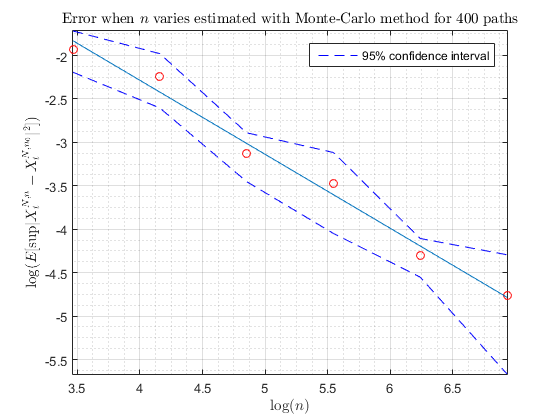
\includegraphics[width=9cm]{finalerror.png}
            \captionof{figure}{Estimation of the $L^2$ error of the Euler-Marayuma scheme with a Monte-Carlo method. $400$ paths, $N=5$, $n\in \{2^5,2^6,2^7,2^8,2^9,2^{10}\}$, reference solution with $n_0=2^{12}$ points.}
        \end{center}
    
    We observe a numerical convergence rate of $0.85$ when Theorem \ref{leo} shows a theoretical rate of $0.5-\varepsilon$.
 
\bibliographystyle{abbrv}
\bibliography{pre}
    
\end{document}